\documentclass[9pt,twocolumn,twoside]{pnas-new}

\usepackage{setspace}
\templatetype{pnasresearcharticle} % Choose template 
\usepackage{fontawesome}
%\usepackage{hyperref}

%\title{Decrypting MINFLUX}
\title{At the molecular resolution with MINFLUX?}

\author[a,b,*]{Kirti Prakash}

\affil[a]{National Physical Laboratory, TW11 0LW Teddington, UK}
\affil[b]{Department of Chemistry, University of Cambridge, CB2 1EW Cambridge, United Kingdom}
\affil[*]{Correspondence: kirtiprakash2.71@gmail.com, \faTwitter  \href{https://twitter.com/kirtiprakash25}{kirtiprakash25}}


\keywords{MINFLUX $|$ STED $|$ SMLM $|$ localisation precision $| $ image resolution $| $ super-resolution imaging} 

\begin{abstract}

\onehalfspacing

\cite{gwosch2020minflux} and \cite{balzarotti2017nanometer} purport MINFLUX as the next revolutionary fluorescence microscopy technique claiming a spatial resolution in the range of 1-3 nm in fixed and living cells. Though the claim of molecular resolution is attractive, I am concerned whether true 1 nm resolution has been attained. Here, I compare the performance with other super-resolution methods focussing particularly on spatial resolution claims, atypical image rendering, visualisation enhancement, subjective filtering of localizations, detection vs labelling efficiency and the possible limitations when imaging biological samples containing densely labelled structures. I hope the analysis and evaluation parameters presented here are not only useful for future research directions but also microscope users, developers and core facility managers when deciding on an investment for the next `state-of-the-art' instrument.

\end{abstract}


\begin{document}

% Optional adjustment to line up main text (after abstract) of first page with line numbers, when using both lineno and twocolumn options.
% You should only change this length when you've finalised the article contents.
\verticaladjustment{2pt}

\maketitle
\thispagestyle{firststyle}
\ifthenelse{\boolean{shortarticle}}{\ifthenelse{\boolean{singlecolumn}}{\abscontentformatted}{\abscontent}}{}

\onehalfspacing
\section*{Introduction}
\noindent
The spatial resolution of light microscopy is continuously being pushed with the development of new technologies. The significant milestones have been confocal laser scanning microscopy \citep{minsky1988memoir}, 2-photon microscopy \citep{denk1990two}, 4Pi microscopy \citep{hell1994measurement}, stimulated emission depletion (STED) microscopy \citep{hell1994breaking}, zero-point STED \citep{baer1999method}, structured illumination microscopy (SIM) \citep{heintzmann1999laterally, gustafsson2000surpassing} and single-molecule localisation microscopy (SMLM) \citep{lidke2005superresolution, betzig2006imaging}. Recently, hybrid super-resolution microscopy techniques have further pushed the spatial resolution down to a few nanometers. These can be further divided into direct combinations of SMLM+STED (for scanning the position of the molecule with a donut) as in MINFLUX \citep{balzarotti2017nanometer} and SMLM+SIM as in SIMFLUX \citep{cnossen2020localization, jouchet2019nanometric} or sequential correlative combinations of SIM and SMLM \citep{rossberger2013combination} and STED and SMLM \citep{Prakash121061}.

The major advantage of the direct combination is in resolution enhancement by increasing the information per photon. For readers interested in the technical details of these methods, following are some excellent recent reviews on this topic \citep{reymond2020modulation, schermelleh2019super, sahl2017fluorescence}. MINFLUX and SIMFLUX have demonstrated a resolution of less than 10 nm on synthetic structures like DNA origami and over 40 nm on biological structures. However, as most of the biologically relevant structures are novel and lie between 10-200 nm range, sequential correlative methods have a distinct advantage to independently validate new morphological findings using an orthogonal technique with a reasonably close resolution.\\  
MINFLUX is presently the most photon efficient method to localize molecules and the aim of this article is not to argue otherwise. Here, I evaluate MINFLUX on the following five broad categories:

\begin{singlespace}
\setstretch{.75}
\begin{enumerate}
\item New biological insights through molecular resolution
\item Apriori structural information and subjective event filtering
\item Atypical image rendering and visualisation enhancement
\item Multi-colour, 3D, live imaging and the caveats when imaging ideal, well-defined structures
\item Spatial resolution vs localisation precision
\end{enumerate}
\end{singlespace}
\noindent
I hope this detailed categorisation helps scientists to evaluate whether MINFLUX is the right microscopy technique for their research. 


\begin{figure}[h!]
\begin{center}
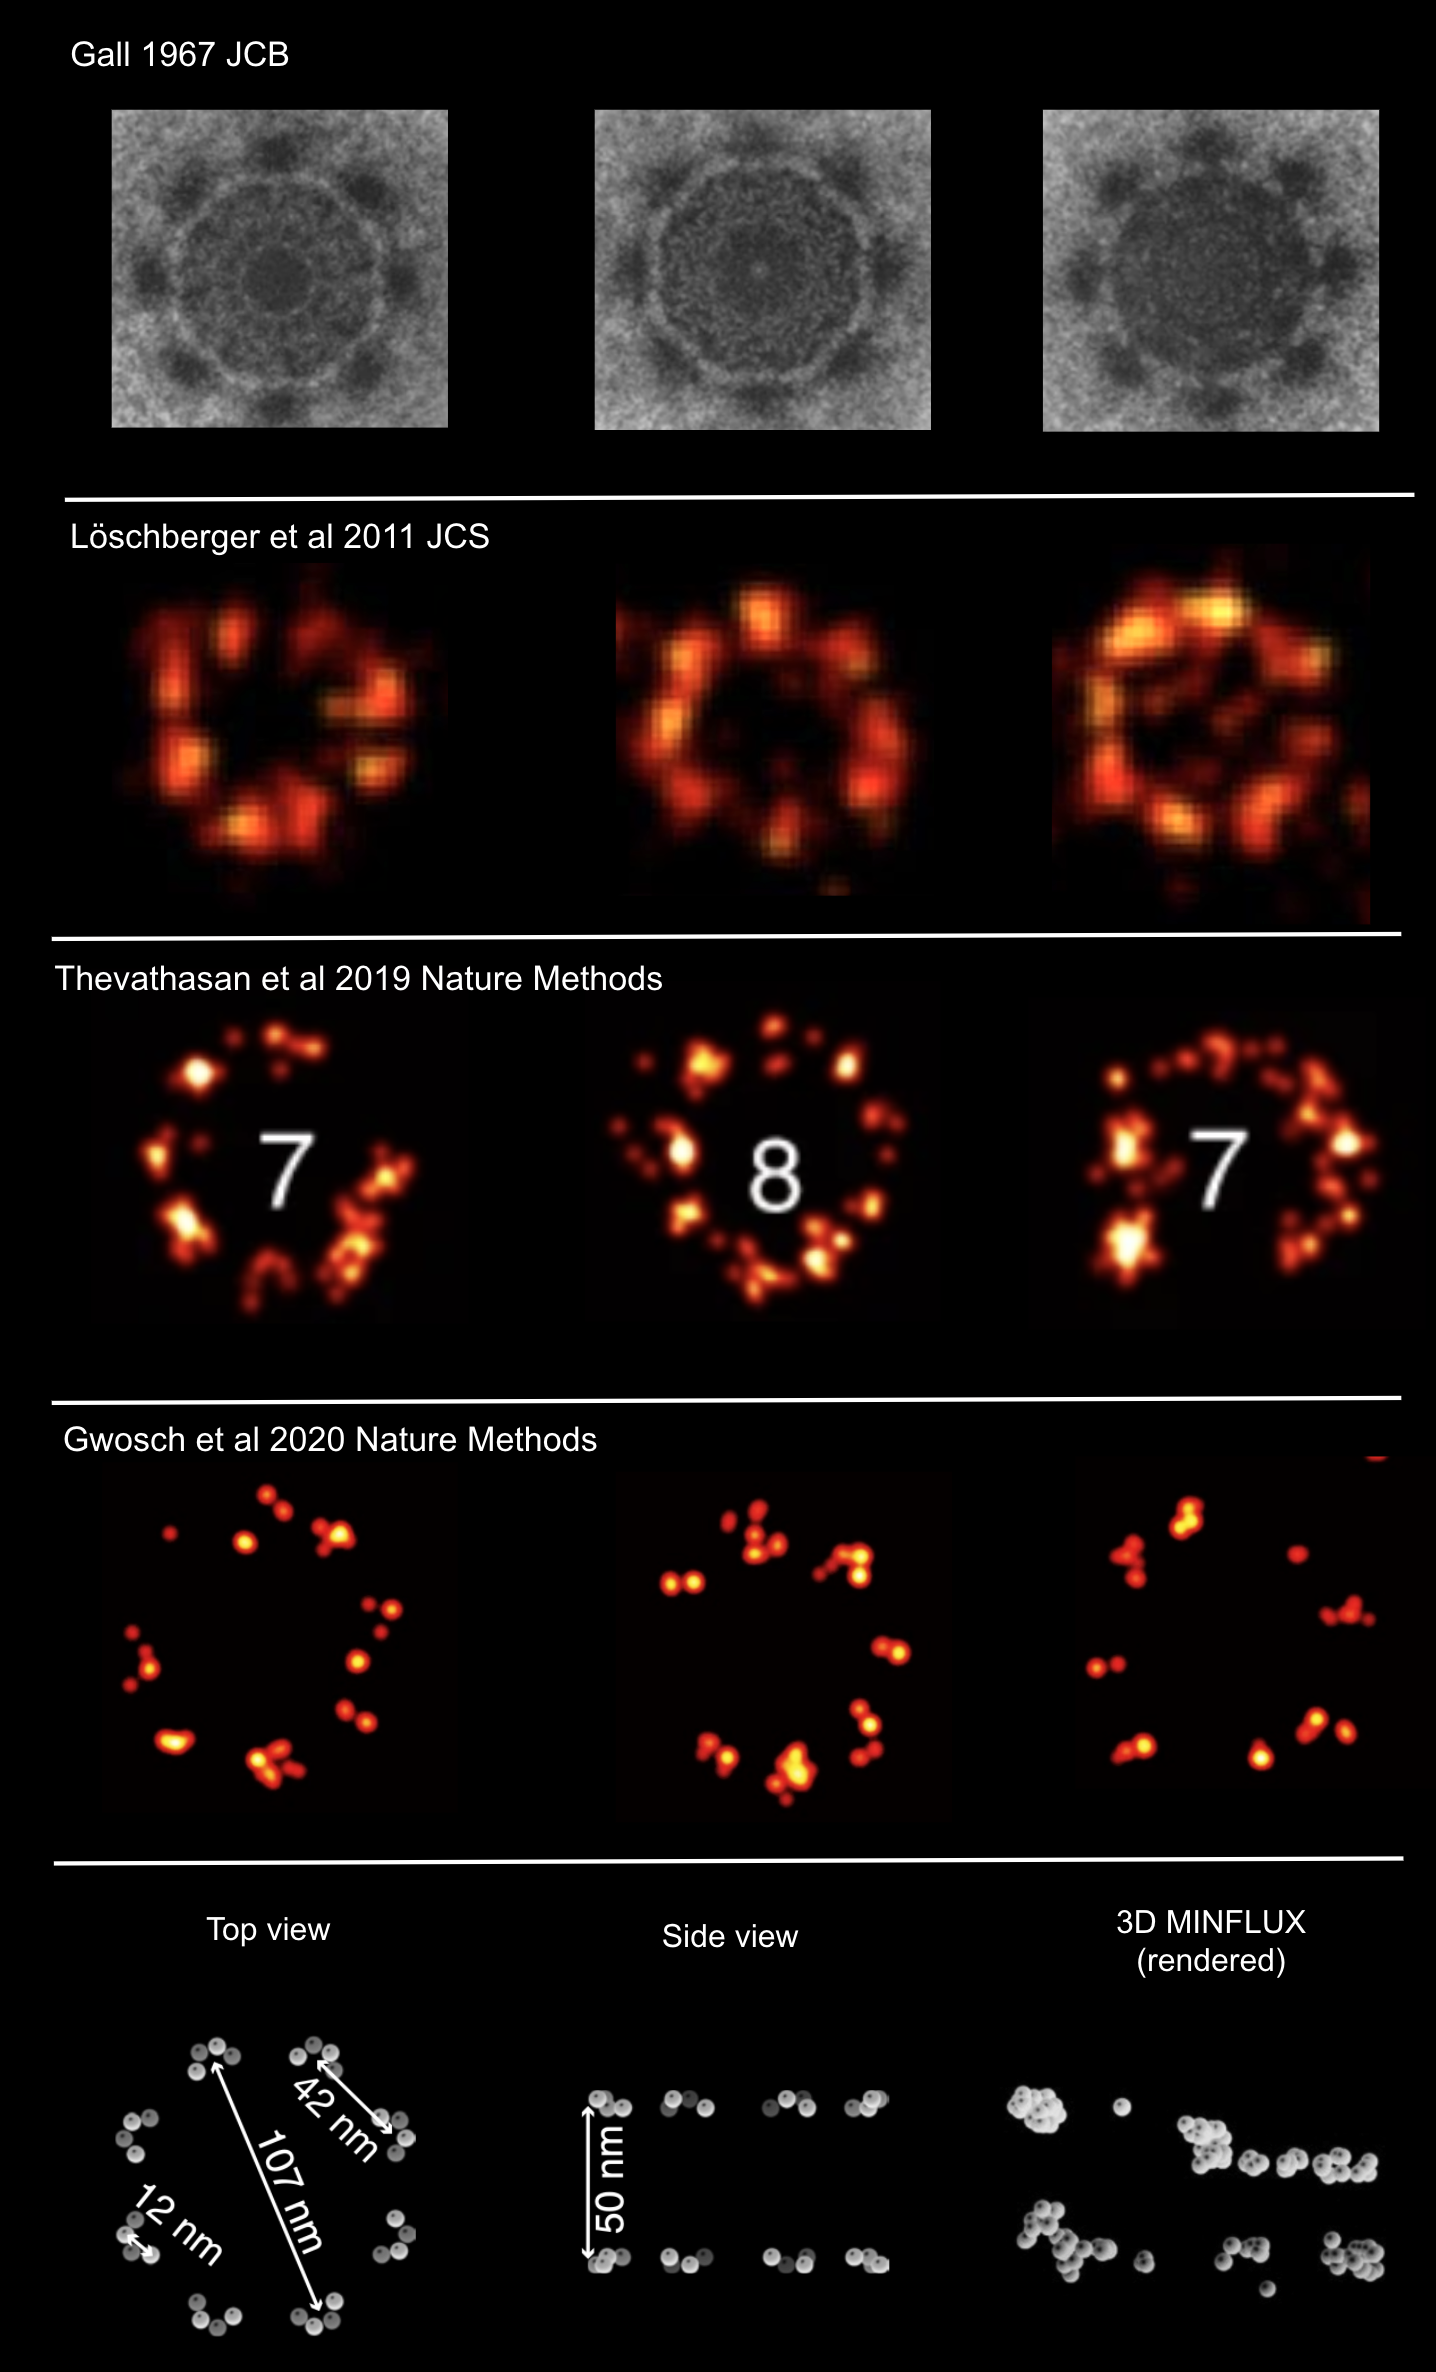
\includegraphics[width=\linewidth]{Figures/NPC2}
\end{center}
\caption[]{\textbf{The need for molecular resolution? Nuclear pores across different imaging modalities}: \\
\textbf{(First row)} Nuclear envelope from amphibian oocyte imaged with electron microscopy. The 8-fold symmetry of the nuclear pores is visible. The pore perimeter shows up as an octagon. Image adapted from \cite{gall1967octagonal}.\\ 
\textbf{(Second row)} Membrane protein gp210 from amphibian occytes imaged with dSTORM (Alexa Fluor 647). The 8-fold symmetry and the circular structures of NPCs is generally seen. The outer diameter is $\sim$120 nm and FWHM of gp210 is $\sim$30 nm. Image adapted from \cite{loschberger2012super}. \\
\textbf{(Third row)} Nup96 endogenously labelled with SNAP-tag (Alexa Fluor 647) in U2OS cell lines. 8- and 7-component pores are more commonly observed. The effective labelling efficiencies for SNAP-Alexa Fluor 647 was $\sim$60\%. Image adapted from \cite{thevathasan2019nuclear}. \\
\textbf{(Fourth row)} MINFLUX imaging of U2OS cell expressing Nup96–SNAP labelled with Alexa Fluor 647. 
6- and 7- component nuclear pores are more prominent raising questions on detection efficiency of the method. A special image rendering was used to visualise the 4 individual copies per subunit of NPCs, which appears as a blob for multi-color MINFLUX imaging, see Figure~\ref{fig:npcs3}. Cell line and labelling strategy same as in  \cite{thevathasan2019nuclear}. Image adapted from  \cite{gwosch2020minflux}. \\
\textbf{(Fifth row)} A schematic of NPCs with the dimensions Nup-96, taken from \cite{thevathasan2019nuclear}.  A 3D MINFLUX `rendered' data presented for comparison from \cite{gwosch2020minflux}. Colormap removed for a fair comparison. Notice the highly clustered, under-sampled and uneven distribution of well-defined periodic nuclear pores. } \label{fig:npcs2}
\end{figure}


\begin{figure}[h!]
\begin{center}
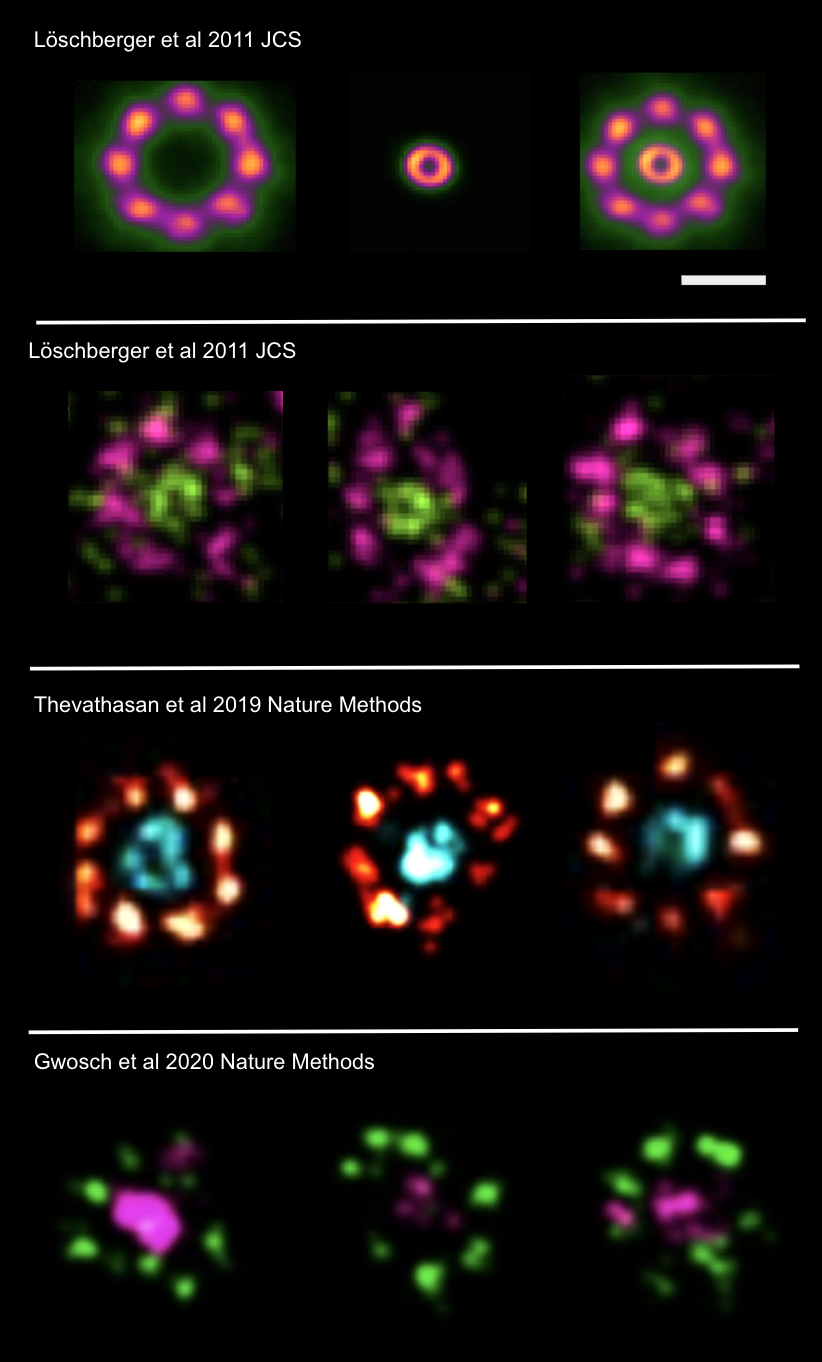
\includegraphics[width=\linewidth]{Figures/NPC3_v2}
\end{center}
\caption[]{\textbf{The missing molecular components with two-colour MINFLUX imaging}:\\
\textbf{(First row)} Schematic for gp210 (the outer ring) and WGA (the central channel) of the NPC. 
The outer ring (gp210) has an average diameter of $\sim$120 nm. The diameter of the inner ring (WGA) is $\sim$40 nm. Image adapted from  \cite{loschberger2012super}.  Scale bar: 100 nm. \\
\textbf{(Second row)} dSTORM images of WGA labelled with ATTO 520 (green) and gp210 labelled with Alexa Fluor 647 (pink) in amphibian oocytes. Both the outer ring and inner channel are visible \citep{loschberger2012super}. \\
\textbf{(Third row)} Two-color SMLM image of Nup96-SNAP labelled with Alexa Fluor 647 (red) and WGA-CF680 (cyan) in U2OS cell lines. The outer ring is clearly visible and the inner ring is also visible in most cases. Image adapted from \cite{thevathasan2019nuclear}. \\
\textbf{(Fourth row)} Two-color MINFLUX imaging of U2OS cell expressing Nup96–SNAP labelled with Alexa Fluor 647 and WGA conjugated to CF680.
The outer ring where each of 8 NPC subunits have 4 copies (as in  Figure~\ref{fig:npcs2}), now appear as a blob. The inner ring (WGA) also aggregates as blobs. Image adapted from \cite{thevathasan2019nuclear}. } \label{fig:npcs3}
\end{figure}


\section{New biological insights through molecular resolution?}

The primary highlight of \cite{gwosch2020minflux} paper is the ability to resolve the individual components of nuclear pore complexes (NPCs) at the molecular scale (Figure~\ref{fig:npcs2}, fourth row). NPCs have eight subunits, each with 4 copies of Nup96 and MINFLUX claims to have  the resolution to resolve these 4 copies. Here, I re-examine this claim to probe if this molecular resolution provided new biological insights or was simply a visualisation enhancement scheme?  

\subsection{New insights into nuclear pore biology}
NPCs are symmetrical structures of eight subunits arranged in an octagonal geometry with an outer diameter of approximately 120 nm (see Figure~\ref{fig:npcs2}, fifth row for a detailed schematic). There are 32 copies of Nup96 per NPC with each of the 8 subunits having 4 copies. These 4 copies are roughly around 12 nm in diameter. The organisation of the 4 copies in the individual subunits is still unknown. With a 1-3 nm resolution range of MINFLUX, a general expectation is to gain structural insights into the organisation of individual components of the NPCs. Do the 4 copies have some ordered organisation (for example, a tetrahedron) or are they randomly distributed? As no observation on the internal organisation of these copies (12 nm structures) are made, it raises questions on the actual usefulness of 1-nm resolution of MINFLUX to provide new structural insights. 


\subsection{Need for independent validation}
It is worth noting that no independent validation of molecular copies or subunits of NPCs was done in \cite{gwosch2020minflux} using either STED or SMLM. Moreover, \cite{thevathasan2019nuclear} used the same cell line (U2OS) and labelling strategy (Nup96-SNAP) as in \cite{gwosch2020minflux} (same authors) and provides an easy basis for direct comparison. The molecular components are 12 nm in diameter and 42 nm apart, so should be easily resolved by SMLM. \\
As far as the organisation of 8 subunits of NPCs is concerned, they have been resolved with electron microscopy (EM) and single-molecule localisation microscopy (SMLM) roughly 50 and 10 years ago, respectively \citep{gall1967octagonal, loschberger2012super}. For a comparison of NPCs using EM and SMLM see Figure~\ref{fig:npcs2}. 

\subsection{Detection vs labelling efficiency}

\cite{gwosch2020minflux} used Nup96 endogenously labelled with SNAP-tag (Alexa Fluor 647) in U2OS cell lines, same as in \cite{thevathasan2019nuclear}. As a general observation, 2-3 components per pore are often missing in MINFLUX data (Figure~\ref{fig:npcs2}, fourth row). MINFLUX images show NPCs with 6- and 7- components, which is not the case with SMLM data. This raises concerns on the detection efficiency of MINFLUX and role of event filtering (see next section). If the missing components are due to labelling efficiency of SNAP-tag then this would be observed in the SMLM data of \cite{thevathasan2019nuclear}. Moreover, if the lack of labelling would be random, 1-2 copies of Nup96 would be missing per subunit of the pore, reducing the intensity but not the entire NPC subunit. Lastly, it is very likely that the subjective filtering of localisations based on photon counts and the distance from the estimated position (structure assumption) leads to the missing of the whole pore subunit. 

\subsection{MINFLUX and the case of fewer photons}

 \cite{gwosch2020minflux} state that MINFLUX requires fewer detected photons when compared to camera-based localization methods like PALM/STORM. So it is applicable to a large range of fluorophores and labelling strategies and is  "bound to be a cornerstone, if not the vanguard, of nanometer-scale fluorescence." However, as of now, MINFLUX has made use of one of the brightest and the best fluorophores for localisation microscopy namely Alexa Fluor 647 and has not done any systematic comparison between dyes or different super-resolution methods. In \cite{balzarotti2017nanometer} MINFLUX comparison with PALM/STORM (using DNA origami) was only a simulation and no experimental data was presented. It is worth noting that the authors as part of another paper \citep{thevathasan2019nuclear} created four cell lines for Nup96 which also includes mEGFP. mEGFP emits relatively lesser photons than Alexa Fluor 647 and the fewer photon claim can easily be tested using this dye. 

 \begin{figure*}[!ht]
\begin{center}
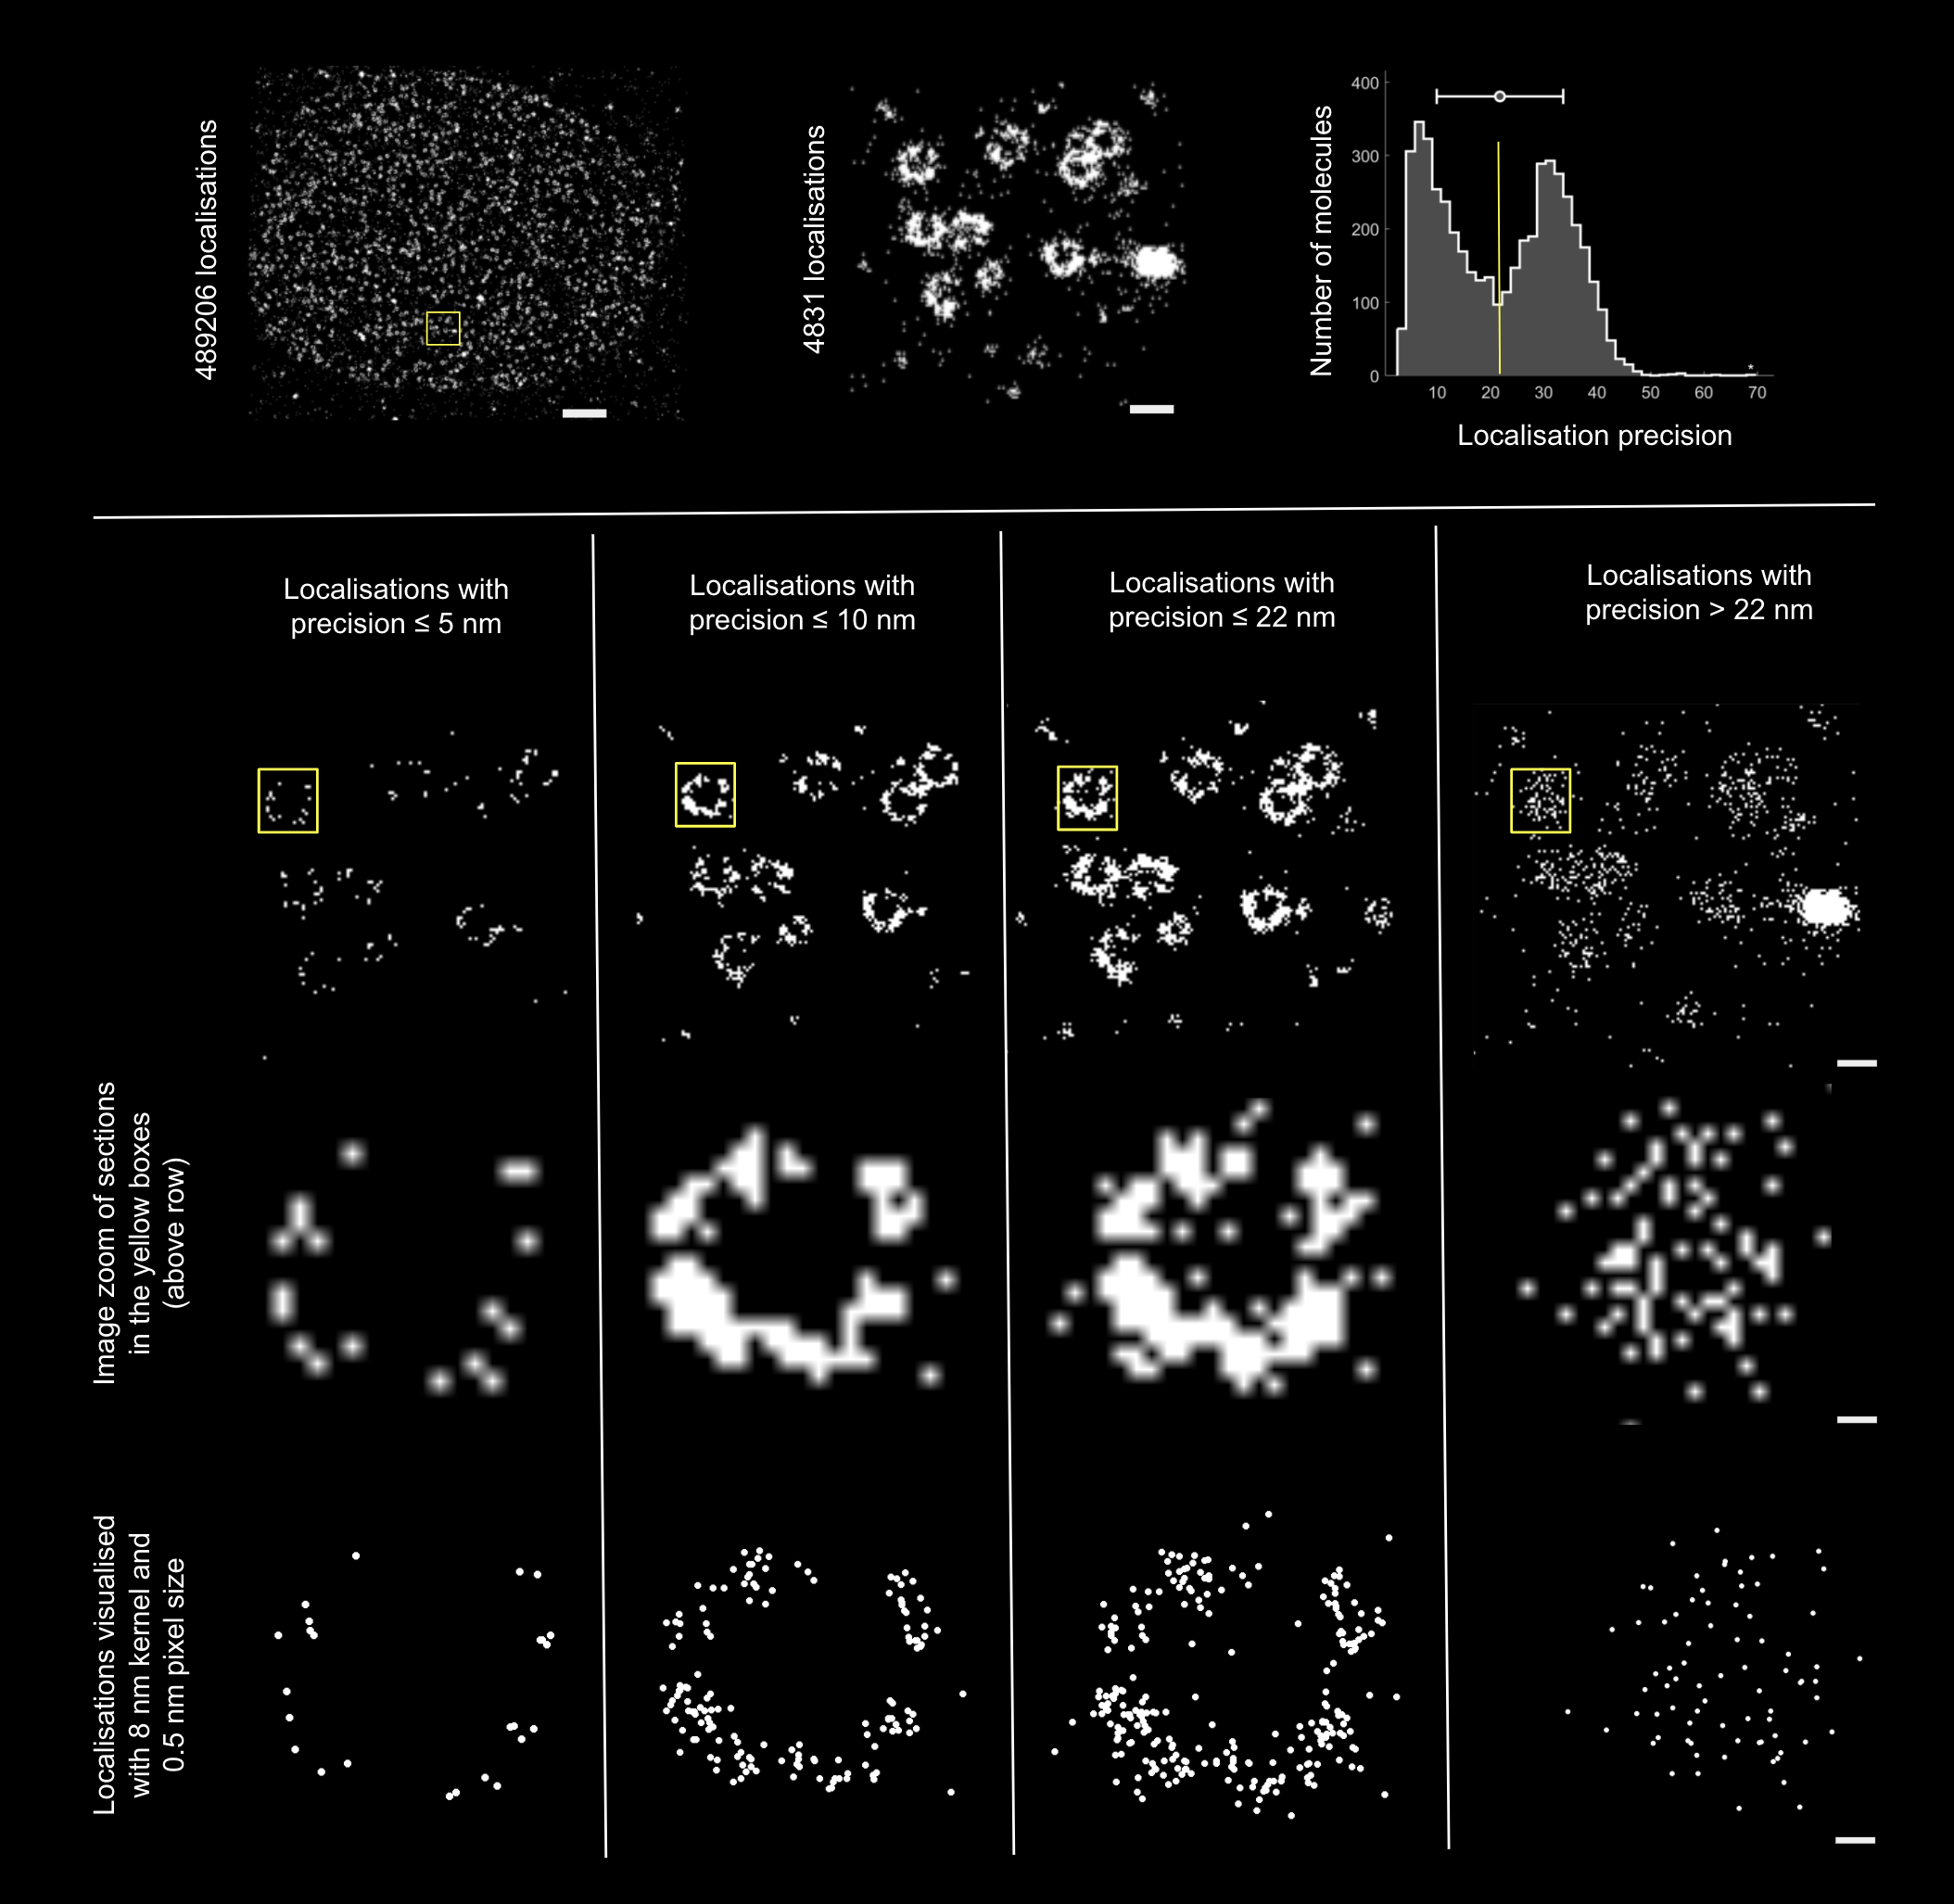
\includegraphics[width=17cm]{Figures/Filtering}
\end{center}
\caption[]{\textbf{Filtering of localisations, visualisation enhancement and molecular resolution:}  \\
\textbf{(Top row)} (Left) Nuclear pore complexes (NPCs) data from \cite{thevathasan2019nuclear}, accessed from \url{https://www.ebi.ac.uk/biostudies/BioImages/studies/S-BIAD8}.  Scale bar: 1000 nm. (Middle) A zoomed-in excerpt (yellow box) with 4831 localisations for further downstream analysis in the panels below. Scale bar: 100 nm. (Right) The localisation precision plot for the zoomed-in excerpt, notice the bimodal distribution. \\
\textbf{(Bottom row, all columns)} The same nuclear pore section with different filtering of localisations at a manually chosen threshold (Scale bar: 100 nm). The zoomed-in excerpts of individual pores (yellow box) highlight the impact of visualisation and image rendering (Scale bar: 10 nm). Notice how the individual components of the 8 subunits of NPCs which can not be resolved with Gaussian blurring, can now be resolved with a manually chosen pixel size and Gaussian kernel (bottom row). The choice of pixel size, Gaussian kernels were done with a prior understanding of how the NPCs `should' look like. The filtering threshold for localization precision was chosen to provide a close to 4 copies per subunits. Often, in such cases, the missing copies are attributed to the limited efficiency of the labelling method.  
 }
  \label{fig:npcs4}
\end{figure*}


\section{Apriori structural information and event filtering}

For years, in electron and single-molecule localisation microscopy, filtering of imaging data has been done to enhance contrast and optimise visualisation. In this section, I highlight how event filtering can be used to attain higher precision computationally, purport new biological structures not present in the raw data and the need for blind samples to standardise the resolution claims.  

\subsection{Localisation filtering at manually defined positions}
To highlight the role of localisation filtering and apriori information to achieve molecular resolution, I use nuclear pore data from \citep{thevathasan2019nuclear}, available at \url{https://www.ebi.ac.uk/biostudies/BioImages/studies/S-BIAD8}.
For downstream analysis at individual nuclear pore level, I zoomed-in at an image section with 4831 localisations (Figure~\ref{fig:npcs4}). For these localisations, the observed bimodal precision plot (centre at 22 nm) was used for further filtering of localisations. The same nuclear pore section with different filtering of localisations at a manually chosen threshold is shown in the bottom row, all columns (Figure~\ref{fig:npcs4}). \\
A single nuclear pore (yellow box) is further highlighted to show the impact of visualisation and image rendering. Notice how the individual components of the 8 subunits of NPCs cannot be resolved with image zoom but can be resolved with a manually chosen pixel size (0.5 nm) and Gaussian kernel (8 nm). The choice of pixel size and Gaussian kernels were done with a prior understanding of how the NPCs `should' look like. The filtering threshold (5 nm) was chosen to provide a close to 4 copies per subunits. Can the missing copies now be attributed to the limited efficiency of the labelling method?


\subsection{The raw and filtered data}
A less-noticed aspect of MINFLUX papers is the almost complete lack of raw data (information about single photons). The only `raw data' presented is filtered and has gone through heavy post-processing. The filtering is done at various levels based on photon counts, targeted coordinate pattern to account for true emission and those considered as background events. For a fair comparison, both raw and filtered data should be presented to demonstrate that any such filtering is not biased by apriori structural information. For structures with prior information like NPCs, the manual filtering can lead to additional biases for live imaging, see Figure~\ref{fig:micos}B. For structures with little prior information, the reduction in the number of molecules would lead to under-sampled structure (Figure~\ref{fig:micos}A). Furthermore, it raises questions on the authenticity of the structures if an independent validation via electron microscopy or other super-resolution methods is not provided.\\
Lastly, it is not clear if the molecular components of NPCs will still be visible in raw/unfiltered data as the increased density of signals will tend to overlap like in the two-colour images (Figure~\ref{fig:npcs3}). Worth noting that subjective manual filtering with better localised molecules (as in Figure S4 of \cite{gwosch2020minflux}) leads to an increased resolution estimate (see Figure~\ref{fig:pminflux} for a comparison). 

\begin{figure}
\begin{center}
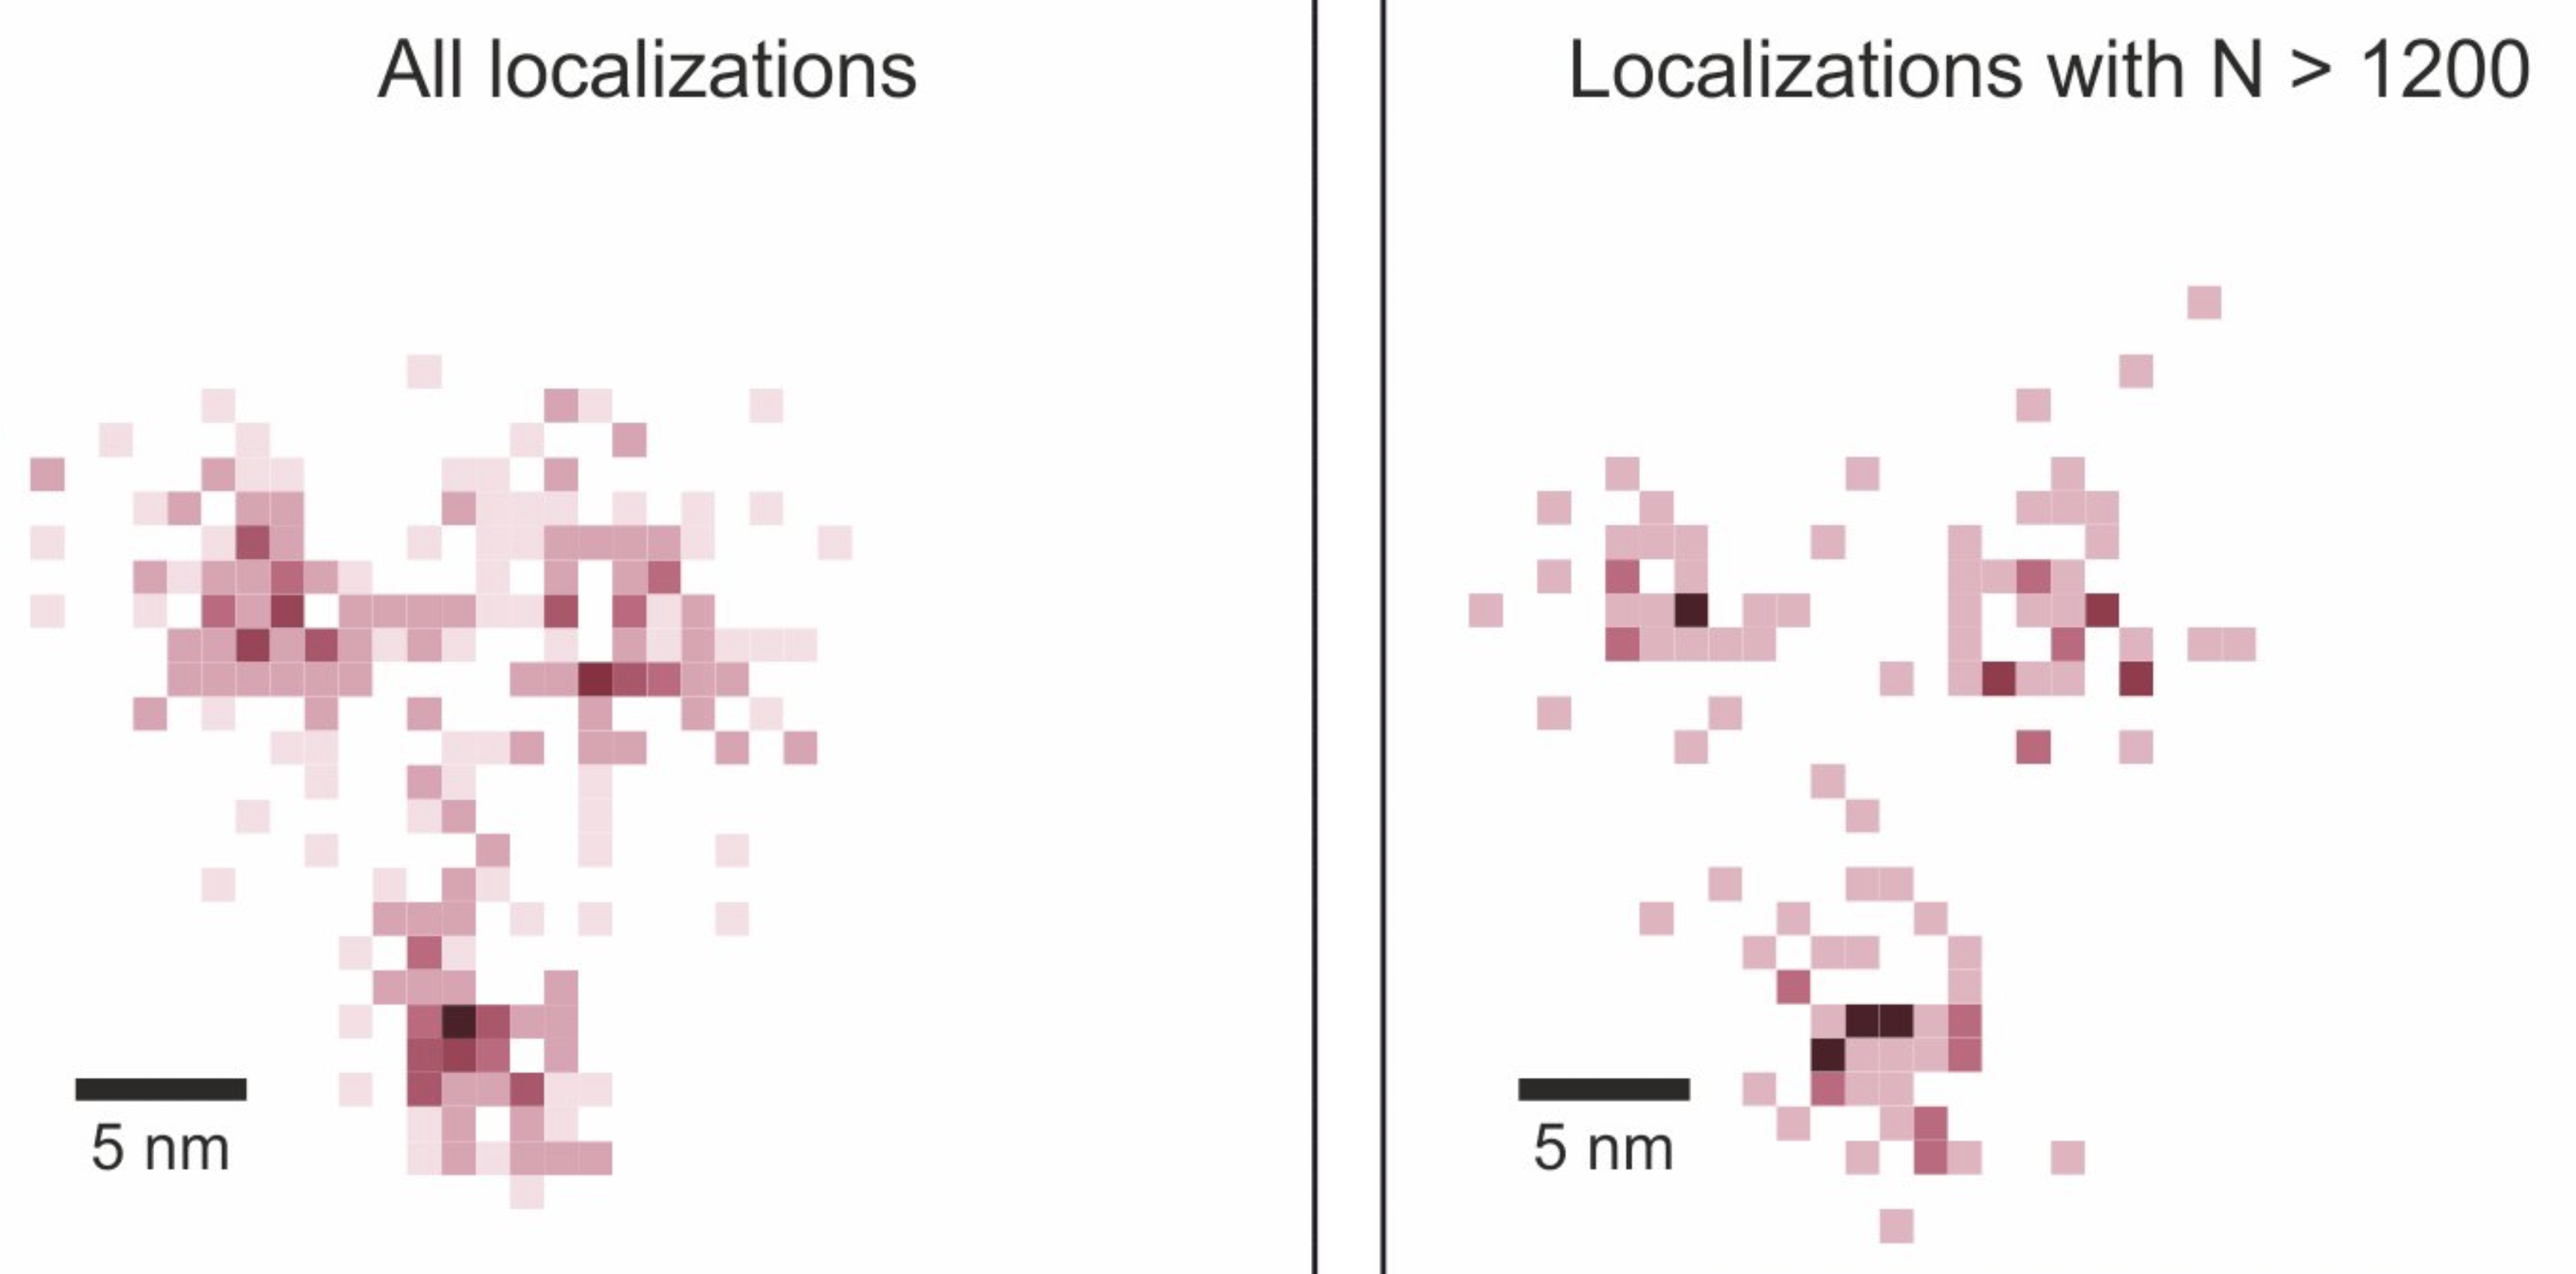
\includegraphics[width=\linewidth]{Figures/pmin}
\end{center}
\caption[]{\textbf{MINFLUX WYAKIWYG: what you already know is what you get:} \\
To demonstrate the difference between the experimental precision and the precision of the filtered data, I use p-MINFLUX data \citep{masullo2020pulsed} provided by Florian Steiner.  Note that the raw data from \cite{gwosch2020minflux} is not publicly available or after reasonable request. \\
 \cite{masullo2020pulsed} state that to achieve a certain precision (2 nm), a minimum number of photons (>1200) are needed and is the primary reason for the choice of filtering threshold. For most biological samples, the underlying structure is almost always unknown, unlike here where the arrangement of DNA origami in 3-dots is known in advance.  This can lead to subjective filtering thresholds for higher spatial resolution claims as long as 3-dots can still be distinguished. What if the arrangement of DNA origami was a T or Y shape, would the same filtering with events >1200 photons be still done?\\
I recommend use of blind samples with no knowledge about the prior arrangement of DNA origami for proper resolution calibration.\\ 
Note that the average precision of all the localizations would be much higher and this number has not been reported by the authors. The precision of all localisations is the true precision of the instrument and not the one calculated on the filtered data.\\
} \label{fig:pminflux}
\end{figure}

\subsection{DNA origami and the need for blind samples}

DNA-origami is commonly used to measure the spatial resolution for different microscope setups. DNA origami has a pre-defined arrangement and blind samples with no knowledge on the prior arrangement are needed for proper calibration. This will make the photon count based filtering  more accountable as origami samples, unlike biological samples, have almost zero background (see Figure~\ref{fig:pminflux}). 
As signal-to-noise ratio is arguably the most important aspect in biological imaging, the effectively achieved resolution is heavily dependent on it and and can vary across sample regions. It is important to understand that unlike an implied single maximum resolution value, the effective resolution is variable, in particular due to the fluctuating contribution of light scatter and out-of-focus blur in different sample regions within the field of view. \\
Results obtained by imaging and analysing DNA origami will likely be a poor predictor of performance for real biological samples where problems of out-of-focus blur, non-specific background, light scattering and other sample aberrations exist. Thus, the resolution claimed based on DNA origami needs to be thoroughly investigated in this context and efforts made not to mislead the researchers interested in real biology. \\
In fact, a new quality metrics for microscopy techniques of the relative deviation between nominal and real life resolution in different biological situations needs to be introduced. After all, conventional fluorescence microscopy rarely achieves its theoretical limit. However, the relative deviation is much smaller than in MINFLUX. 

\subsection{The choice of biological sample for resolution claims}
For the lateral spatial resolution, so far, MINFLUX imaging has been done on NPCs \citep{gwosch2020minflux}, mitochondrial MICOS proteins \citep{pape2020multicolor} and post-synaptic protein PSD-95 \citep{gwosch2020minflux}. These can be classified as samples having a well-defined underlying structures (NPCs) or with no inherent underlying structures (MICOS, PSD-95). 

For the biological targets with no underlying structure, an independent validation with another super-resolution method or a relative comparison under identical imaging conditions and length scales is essential. For such studies, a minimum signal density and labelling efficiency should be considered as a minimum requirement.\\
For the biological targets with an underlying organisation such like NPCs, the filtering of data can be misused to attain a certain resolution (see Figure~\ref{fig:pminflux}). Furthermore, such filtering would lead to biases in labelling and detection efficiency. 
 

\begin{figure}[!ht]
\begin{center}
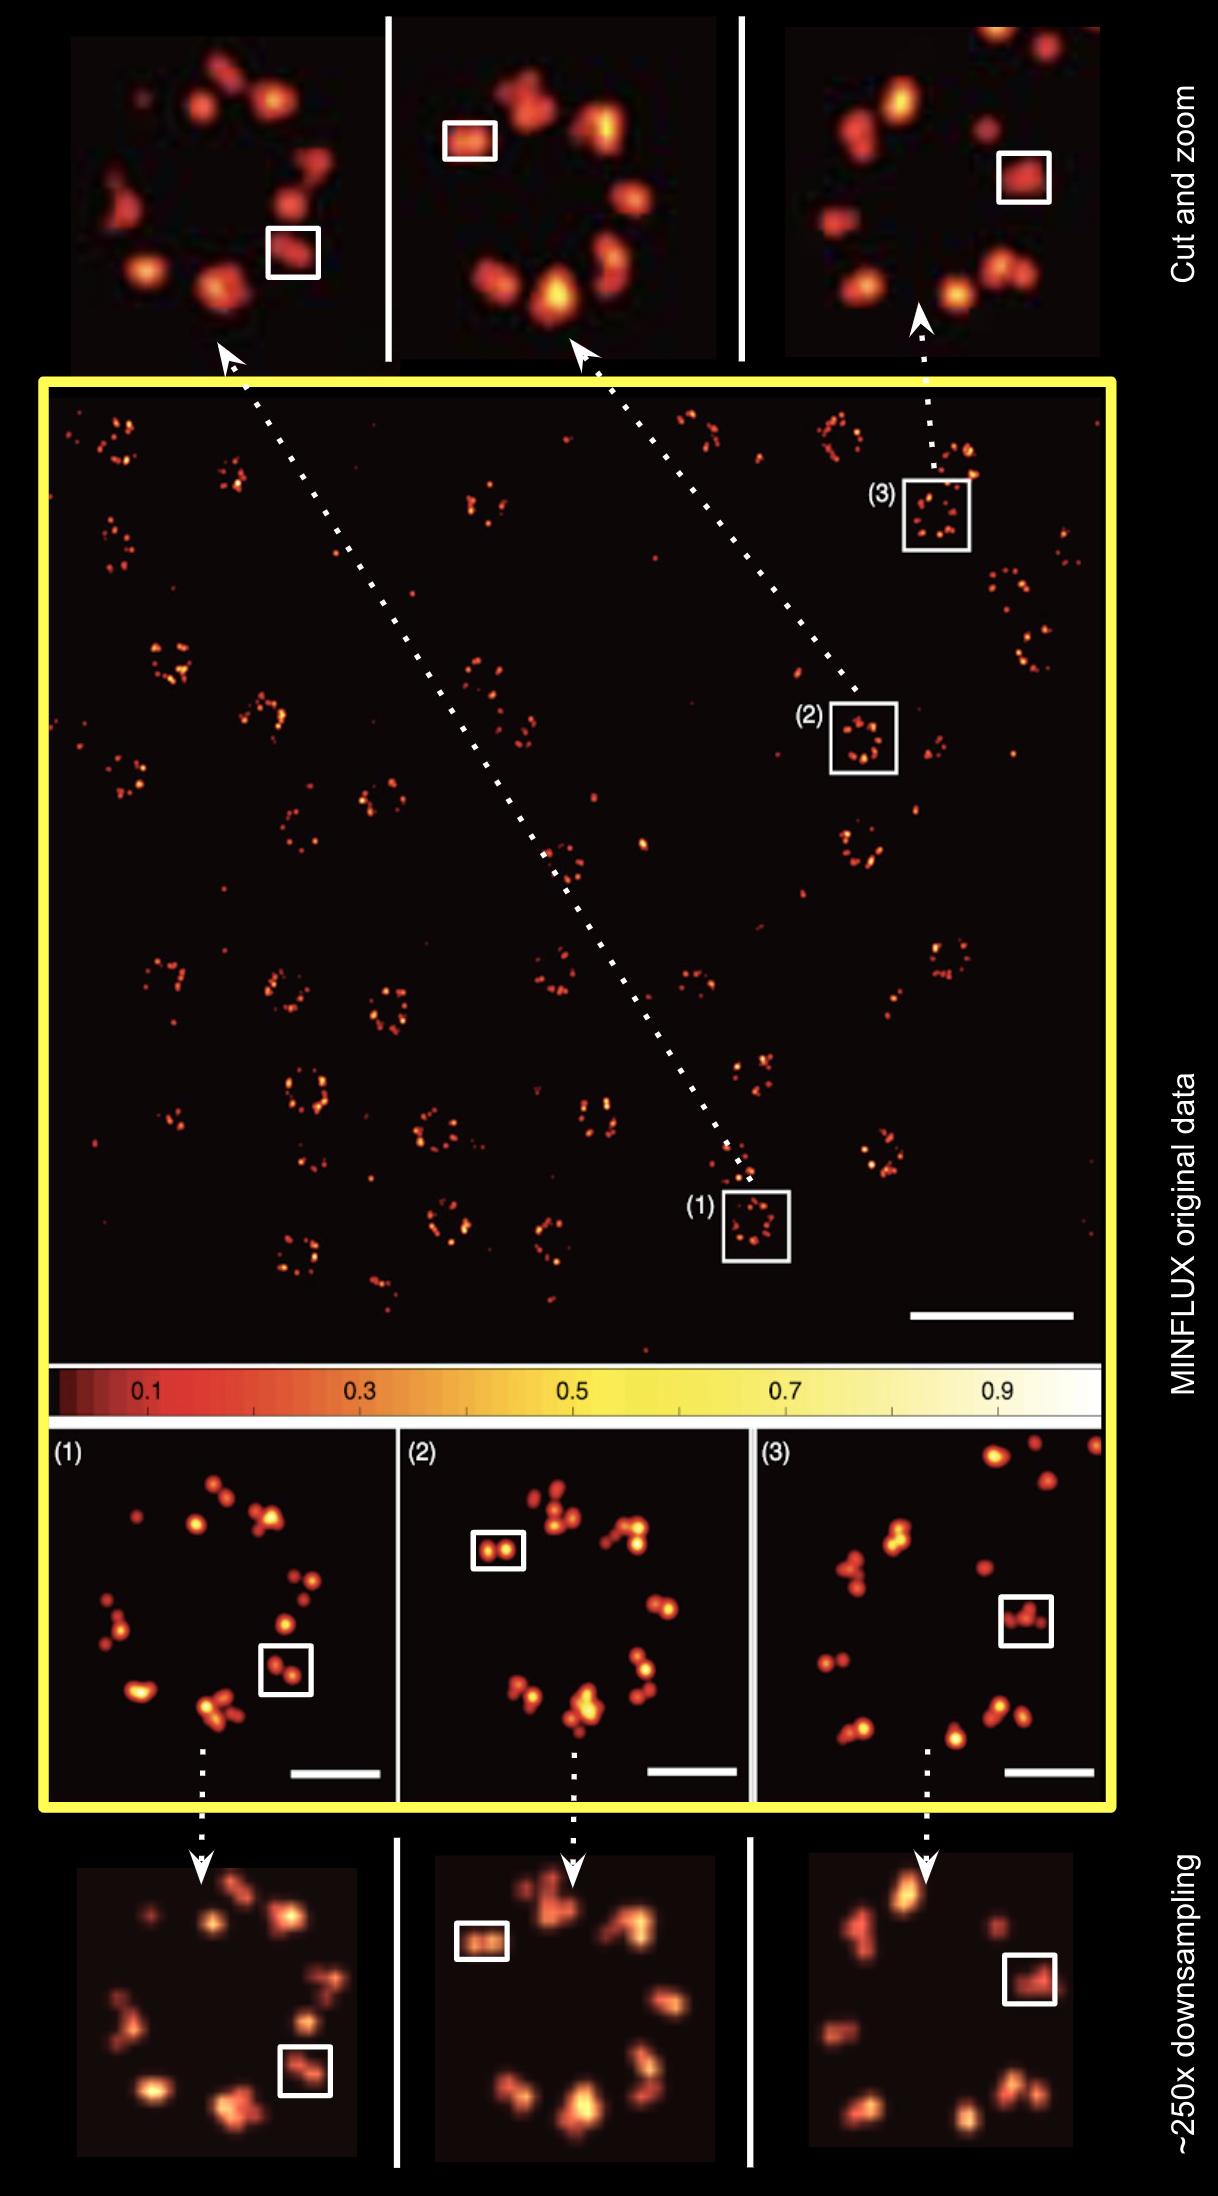
\includegraphics[width=8.4cm]{Figures/NPC1}
\end{center}
\caption[]{\textbf{Visualisation enhancement and image rendering:} \\
\textbf{(Top row)} The zoomed in sections of inset (1), (2) and (3) from the yellow box below.\\
\textbf{(The yellow box)} U2OS cell expressing Nup96–SNAP labelled with Alexa Fluor 647 taken from \cite{gwosch2020minflux}. Below, zoomed in sections of inset (1), (2) and (3) of Nup96. The data presented here is not the raw data and has gone through several filtering steps. Such filtering is easier when prior information about the structure is assumed. Scale bar: 500 nm for the large field of view, 50 nm for the zoomed in excerpts, also for the top and bottom row. \\
\textbf{(Bottom row)} The section of inset (1), (2) and (3) from the yellow box down-sampled (from $\sim$500*500 to $\sim$32*32, $\sim$250x) to bring at the same level as in the top row. The aim of this reverse engineering is to demonstrate that the image doesn't contain enough information to make the molecules from individual subunits of NPCs visible.\\
\cite{gwosch2020minflux} used special image rendering (different pixel sizes, Gaussian kernels and non-linear color maps) to highlight the individual copies of the 8 subunits of NPCs quoting visibility as the primary reason. The octagonal structure of NPCs (8 subunits) is well-known but not the organisation of individual copies. As no independent validation via electron microscopy or other super-resolution methods was made, I question the validity of such special image rendering to claim the information not present in the raw data. 
} \label{fig:npcs1}
\end{figure}

\section{Image rendering and visualisation enhancement}

In this section, I highlight the special image rendering and visualisation enhancement methods used in MINFLUX and the possible implications. The aim here is to make the readers understand the fine difference when new biological structures like the molecular components of nuclear pores are shown for visual purpose but not to claim any structural biology. 



\subsection{Single-molecule subtleties}
Though MINFLUX increases the localisation precision by improving photon statistics, I believe the observed molecular components (Figure~\ref{fig:npcs1}, yellow box) are a result of atypical image rendering and subjective filtering of the localisations. Over the years, the single-molecule community for visualisation enhancement, rendered the localisation data using a smaller Gaussian, e.g. 5 nm kernel (or localisation precision), even if the average experimental precision was 30 nm. This was exclusively done to make final images more appealing for established biological structures but not to claim new biology. MINFLUX has borrowed several of these subtleties from the single-molecule imaging field but by not presenting the raw data is obscuring the motivation. 

\subsection{Reverse engineering the molecular components}
As the raw data is not available, I down-sampled the images from \cite{gwosch2020minflux} to test if MINFLUX has the potential to optically resolve the molecular components of NPCs. The zoomed-in sections (Figure~\ref{fig:npcs1}, yellow box) had to be downsampled by 250-fold (Figure~\ref{fig:npcs1}, last row) to match with the zoomed-in region of the original image (Figure~\ref{fig:npcs1}, top row). Even with $\sim$250-fold down-sampling, one can better resolve the molecules of the individual components of nuclear pore complexes (NPCs). Given the difference in the sizes of NPCs, I argue that molecular copies of NPCs observed in the zoomed-in sections are not present in the raw data and are rather the result of the image rendering procedure. 

\subsection{Image rendering and the renditions}
For image rendering, the authors used different pixel sizes, Gaussian kernels and non-linear colormaps to highlight the molecular copies of NPCs. For example, a pixel size of 0.5 nm and a large-width Gaussian kernel of 4 nm was used for Figure 2a and 5e but a kernel of 2 nm and a pixel size of 0.2 nm for Figure 2a and 2f in the paper \citep{gwosch2020minflux}. However, the authors state this was done for visibility reasons. In this regard, it is important to observe the renditions of each molecule and the deviations from the rendered data as the raw data is not available. 

\subsection{The devil is in the minutest detail}
Another noteworthy aspect is how the unequal number of events per fluorescent molecule were compensated with a non-linear color distribution. Using non-linear colormaps, all localisations were rendered with the same precision. I believe, this was not done to just improve the visibility but to highlight the `molecular' nature of the method. This becomes obvious when the non-linear colormap is taken away. As an example, see the potential for overlap of molecular components when the localisations would be rendered with the original precision (Figure~\ref{fig:npcs2}, last row). The data taken from \cite{thevathasan2019nuclear} with same labelling strategy as \cite{gwosch2020minflux}. 

\begin{figure*}
\begin{center}
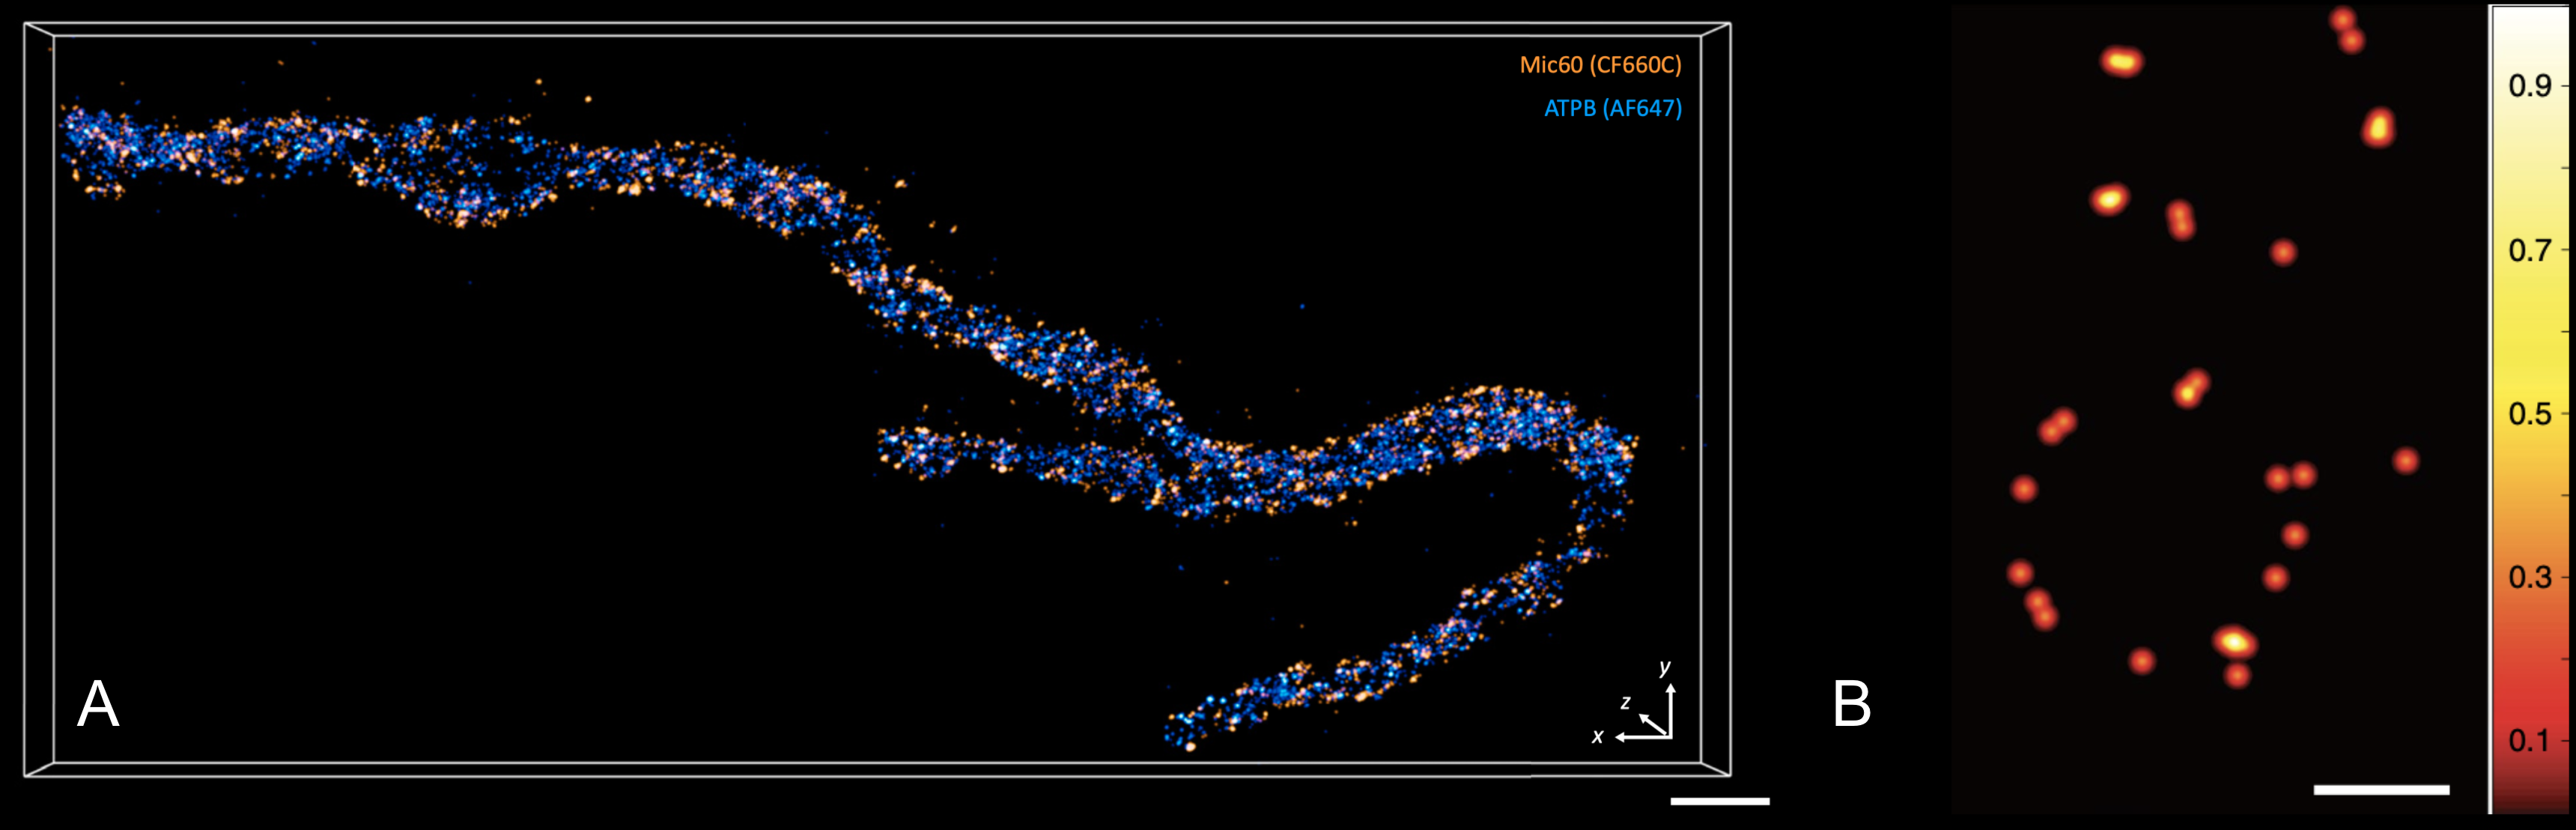
\includegraphics[width=17cm]{Figures/dense}
\end{center}
\caption[]{\textbf{MINFLUX imaging of densely filled ring-like structures of Mic60 and Nup96:} \\
(A) \cite{pape2020multicolor} claim to observe ring-like arrangements of Mic60 molecules with a diameter of 40 to 50 nm. The ring-like arrangement is rather subjective here and is left for the readers to interpret themselves (see  \href{http://movie-usa.glencoesoftware.com/video/10.1073/pnas.2009364117/video-6}{Movie} for more insights). As no independent validation of these ring-like strictures via electron microscopy or other super-resolution methods is provided in the paper, the observed punctuated structures can, at best, be considered as a highly under-sampled ring. This raises questions on the detection efficiency of the method and its ability to image dense as well as continuous structures. Scale bar: 500 nm \\
(B) Live MINFLUX imaging of nuclear pores expressing Nup96–mMaple in U2OS cell. Notice the highly under-sampled configuration of nuclear pores as only the localizations with more than 1600 photons were considered. Image adapted from \cite{gwosch2020minflux}. Scale bar: 50 nm.
} \label{fig:micos}
\end{figure*}



\section{Multi-colour, 3D, live MINFLUX imaging  and caveats when imaging continuous well-defined structures}

MINFLUX was originally published in 2017 \citep{balzarotti2017nanometer} with nanometer resolution claim on a synthetic structure (DNA origami) and particle tracking in bacterial samples. In \cite{gwosch2020minflux}, the authors, for the first time, claim nanometer resolution in biological samples, in three dimensions, in living cells and using multiple color channels.  In this section, I evaluate method's potential and the strength of the reported data (Figure~\ref{fig:micos}).  


\subsection{The missing molecular components in multi-color imaging}
The individual proteins of the eight NPC subunits (roughly 40 nm apart) that can be observed in single-colour images, vanish in two-colour images (Figure~\ref{fig:npcs3}) questioning the performance and resolution claim of MINFLUX  under these imaging conditions. The molecularly resolved 4 copies of the subunits now appear as a `blob' in 2-colour images. This also includes the inner ring of the WGA displayed as a blob in the second colour channel. Note that both the inner and outer ring are clearly visible in  \cite{loschberger2012super} and \cite{thevathasan2019nuclear} respectively. In summary, for 2 colour imaging experiments, MINFLUX appears to offer an effective lateral resolution that is no better than localisation-based super-resolution methods, if not worse (see Figure~\ref{fig:npcs3} for a detailed comparison). Can the molecular resolution still be claimed given that no `molecules' are observed in a 2-colour MINFLUX imaging experiment? 


\subsection{The rendered 3D MINFLUX data}

Regarding the 3D imaging of well-defined structures like NPCs, the rendered MINFLUX data appears to be highly clustered, under-sampled and unevenly distributed (see Figure \ref{fig:npcs2}, fifth row for a comparison with schematic of 3D organisation of NPCs). Several SMLM papers have put out a high-quality 3D structure of NPCs and is difficult to compare them with the rendered data from \cite{gwosch2020minflux}. The under-sampled data again raises questions on detection efficiency of MINFLUX and its applicability for nuclear pore biology. It is also noted that no quantitative comparison of MINFLUX for Z resolution with SMLM is provided. For excellent 3D nuclear pore data, please refer to Figure 1 of \cite{thevathasan2019nuclear}. \\
The two-color 3D images of the nuclear pores with WGA (CF680) and Nup96 (SNAP-Alexa Fluor 647) again are barely comparable with standard 3D SMLM images. The ring distribution of WGA is unresolved and instead appears like a random distribution of points. The Nup96 octamer is also hardly visible, both laterally and axially (see Figure 5 and Supplementary Video 3 of \cite{gwosch2020minflux}). Lastly, given the MINFLUX claim to be applicable to a large range of fluorophores, I wonder the use of CF680 with Alexa Fluor 647 with both excitation and emission spectra overlapping. Both dyes can be reasonably combined using spectral unmixing approach \citep{zhang2015ultrahigh}, however, the motivation to use this pair is missing in the MINFLUX paper. 



\subsection{MINFLUX imaging of continuous well-defined structures}

MINFLUX has been used to probe the sub-mitochondrial localization of the core MICOS proteins \citep{pape2020multicolor}. The authors claim to observe ring-like arrangements with a diameter of 40 to 50 nm. Upon close examination, it appears that ring-like arrangement is rather subjective and the readers are encouraged to interpret it themselves, see Figure~\ref{fig:micos}A and \href{http://movie-usa.glencoesoftware.com/video/10.1073/pnas.2009364117/video-6}{Movie S6} of \cite{pape2020multicolor}. As no independent cross-validation of these ring-like strictures via electron microscopy or other super-resolution methods is provided, it raises concerns on the validity of the observed punctuated structures. These punctuations, at best, can be described as a highly under-sampled ring. At this point, it is not clear if this is due to the detection efficiency of MINFLUX and its limitation to image dense as well as continuous structures. This, in turn, highlights the need for sequential correlative super-resolution methods where new structural findings from one method can be independently validated under similar imaging conditions. Lastly, the claimed localisation precision of 5 nm with a structural resolution of 40-50 nm brings in the debate of the difference between experimental `localisation precision' versus achieved practical `structural resolution' and how these numbers should be reported. \\
\noindent
\textbf{The missing microtubules:}
Historically, FWHM of microtubules (MTs) has been the benchmark for resolution demonstration in STED microscopy. MTs are continuous and have a denser tubular organisation (25 nm) when compared to the nuclear pores. Hence, any subjective filtering would lead to an under-sampled image. 
On the other hand, the hollow tube structure of MTs has been resolved with SMLM and DNA-PAINT setups. For a well resolved 3D cylinders of microtubules with SMLM, see \cite{huang2016ultra,li2018real}. As none of the MINFLUX papers include imaging of MTs, it raises concerns regarding the potential of MINFLUX to achieve the same level of structural resolution and if the technique might be limited to sparse and non-continuous structures. As a side note, to the best of my knowledge, the 25 nm tubular structure of MTs have never been shown even by STED.\\
In summary, MINFLUX performance on continuous structures with a well-defined organisation, such as MTs or those for which prior information is not available, remains to be proven. 
For MICOS, post-synaptic proteins, etc., which do not have an underlying structure, any resolution and shape can be claimed but is it valid?

\subsection{Live MINFLUX imaging}
MINFLUX imaging of nuclear pores (Nup96–mMaple) in living U2OS cells shows a highly under-sampled configuration with no data on cell viability or photo-bleaching (Figure~\ref{fig:micos}B). The observed uneven distribution of nuclear pores is possibly due to heavy filtering of localizations (>1600 photons).\\
Regarding excitation powers for live imaging, the authors used powers $\sim$20-60 $\mu$W with the peak intensities of the donut beam $\sim$10–50 $kW/cm^2$. For single molecule techniques, the excitation power is $\sim$0.1 kW/$cm^2$ to switch the fluorophores between dark and bright state, $\sim$1000-fold less \citep{betzig2006imaging}. For structured illumination and confocal microscopes, especially the laser-free versions, the excitation powers are in tens of $mW/cm^2$ range or below. Thus, for live imaging MINFLUX is still off by a significant margin with respect to excitation powers when compared to single-molecule imaging, structured illumination or confocal microscopy.


\section{Spatial resolution and localisation precision}

MINFLUX nanoscopy claims to provide a "resolution in the range of 1 to 3 nm for structures in fixed and living cells". It is important to remember that 1-3 nm range here refers to localisation precision, and more specifically of fluorophore and not that of the target protein (Figure~\ref{fig:lp}). As argued in this paper, MINFLUX is yet to resolve structures below 40 nm in biological samples. For synthetic structures like DNA origami, subjective event filtering can lead to unrealistically high precision numbers. 

\subsection{Precision is not resolution}
For years, localisation precision and spatial resolution have been interchangeably used by physicists given their inherent dependence on photons. Resolution i.e. the ability to resolve close-by structures or target molecules, primarily depends on how densely a biological structure is labelled while localisation precision implies how well these labels are detected, see Figure~\ref{fig:lp} for more details. \\
For single-molecule studies, localisation precision follows an inverse square-root relationship with the total number of detected photons, whereas MINFLUX has an inverse quadratic relationship with detected photons under ideal conditions with zero background. For real-life biological applications, MINFLUX is severely limited by the background photons as this compromises the positioning of the donut zero. In general, MINFLUX  is likely to achieve better precision numbers than single-molecule imaging but so far, due to multiple reasons stated in this article, the spatial resolution of the method has been much poorer than SMLM methods (see Figure~\ref{fig:npcs2}).  

\subsection{Resolution quantification}
\cite{gwosch2020minflux} applied three different criteria for resolution quantification. The first approach was to calculate the standard deviation for >5 localizations/fluorophore, where each localization had $\sim$2000 photons. The events with high photon counts would automatically result in higher precision numbers. Notice how \cite{gwosch2020minflux} begin with resolution quantification but quote the precision of filtered data, skipping the average precision of all localisations. This leads to confusing localisation precision of a fluorophore with the spatial resolution of the method. \\
The second resolution assessment is by subtracting the mean localized position from all localizations. This process is similar to the first approach and will be biased by the filtering of the data. %was done by ``subtracting the mean localized position of an emission train from all of its single localizations." This .\\
The third approach is based on Fourier ring correlation (FRC) and it is not clear whether filtered or raw data was used for FRC analysis. A proper assessment of spatial resolution and localisation precision is not possible given the unavailability of the raw data and the codes. % available so that a claim of 1-nm can verfied even from a physicists' perspective. 

\subsection{1-nm resolution and 3-nm linker}
From a biochemistry point of view, is it reasonable to claim a resolution in the range of 1-3 nm when the SNAP-tag itself is about 3-3.5 nm in size? Given the resulting uncertainty of relative position of the dye molecule, the stated nanometer resolution (or the localisation precision for that matter) can only be claimed for the fluorophore, but not the biological target. In this context, I urge the readers to take a careful note when authors state the precision of the fluorophore and that of the target protein. 
 
\subsection{Is it all about the principle and not practice?}
Generally speaking, the resolution is the fundamental ability to determine a structure. From a physicist perspective it is satisfying that MINFLUX can achieve 1-nm localisation precision under ideal conditions (based on photon statistics), whether it materialises in resolving real life biology or not. 
From a biologist perspective, for a 1-nm resolution claim, MINFLUX is off by a factor of 5 for synthetic samples like DNA origami and a factor of 40 for biological samples like NPCs. \\
For a true 10-nm strucutral resolution, a general expectation would be to resolve a well-established 10 nm bead-on-string structure of nucleosomes or a turn of DNA helix which is about 3.4 nm (for 1-nm claim). From Nyquist viewpoint to achieve 10 nm structural resolution, one would need a dye every 4 nm, which for many biological structures is hard to achieve due to steric hindrance or low copy number/binding sites. Alternatively, for structural biology, with true 1-nm resolution claim, I wonder if one can compare MINFLUX with X-ray crystallography, which has a broad range of resolution (anything between 1.5 and 10 Å) depending on the crystal quality.



\section{Summary and the lessons from the past}

\subsection{Towards standard biological reference structures}
The spatial resolution in light microscopy has become something of a numbers game where scientists cite an arbitrary FWHM or an FRC resolution or filter localisations to achieve any desired resolution. Given the large number of potential biological reference structures in the range of 1-100 nm size scale, for example, DNA (2 nm), nucleosomes (10 nm), microtubules (20 nm), NPCs (40 nm), synaptonemal complexes (60-150 nm), I recommend using these well-defined structures to support spatial resolution claims. For DNA origami researchers, I encourage usage of blind samples where no one knows the origami arrangement or the distances in advance. This will make the photon count based filtering  more accountable. 

%though a Global FRC is still better then FWHM of a selected sample site, or the misleading localisation precision number.
\subsection{Potential research areas for MINFLUX}
\cite{gwosch2020minflux} and \cite{balzarotti2017nanometer} have made efforts to push the localisation precision to single nm range which works well on ideal synthetic samples, but major compromises need to be made when applying these techniques to real-life biology. MINFLUX has value for a certain specific application (e.g. single-molecule tracking), but in its current state, it should not be considered as the next-generation versatile imaging platform. Technical issues like detection vs labelling efficiency, limitation when imaging for well-defined, continuous and dense structures, the use of well-characterised single-molecule dyes still limits its broader applicability. 

\subsection{Reproduction crisis}
MINFLUX papers have shown several loop-holes in current scientific reporting and standards. A clear distinction needs to be made about experimental precision, spatial resolution, cross-validation of new structures by independent methods, extent of sample variability vs measurement uncertainty, hardware adaptability, image quality/standards (for example, acceptable measures for image rendering), availability of raw data/codes, reproducibility of the analysis pipeline, automated vs manual components of data analysis (like filtering) and proper procedures to report them. \\
From a historical perspective, 4Pi, STED and now MINFLUX have been closed systems with little focus on making the hardware adaptable or raw data/codes available. Several units of highly-priced 4Pi microscopes were sold around 2000s as the next generation microscope, however, not many biological findings resulted. This was followed with the launch of STED microscopes and very few novel biological results. \\%Over the years, the STED community have failed to maintain transparency and create an environment for reproducible science.
Science is about reproducible measurements. Improvement in precision leads to refined measurements. MINFLUX improves the precision with which fluorophores can be localised but by not making the hardware adaptable, raw data and codes available, it is hindering reproducibility, open science efforts and overall progress of the field.  

\subsection{Important conceptual advancement vs current technical limitations} 
One of the important aspects of science is to promote cutting-edge ideas even if they offer little gains in the short run. MINFLUX research provides an important conceptual advancement and leads to overall progress in the field. The aim of this article is not to discourage MINFLUX research but to highlight that the technology is still underdeveloped and needs further validation from other independent labs before it is made commercially available especially considering the high price tag of the commercial system. \\
As research grants mostly come from tight public funds and are a zero-sum game, I hope this critique provides the scientists, microscope users, developers and core facility managers with an alternative viewpoint when deciding about an investment in the next ``state-of-the-art” microscope instrument.  

\section*{Acknowledgements}
I thank Eric Betzig, Johannes Hohlbein, Lothar Schermelleh, Michael J Shaw, Richard W Clarke, Tulika Gupta and Rainer Heintzmann for useful discussion and/or comments on the manuscript. I further thank Alessandro Esposito, Jelmer Cnossen, Alex Merz, Francisco Balzarotti, Seamus Holden, Florian Steiner and Johannes Hohlbein for actively participating in the open public Twitter (\faTwitter) discussion on this topic which can be followed \href{https://twitter.com/kirtiprakash25/status/1336575288122204160}{here.}
%No raw data from \cite{gwosch2020minflux} was made available upon reasonable request. 
I thank Florian Steiner for sharing the image (via Twitter) used for Figure~\ref{fig:pminflux}. 

\section*{Conflict of interest}
The author declares no conflict of interest.

\small
\bibliographystyle{apalike}
\bibliography{mylib}


%\newpage
\onehalfspacing
\onecolumn
\noindent
%\widetext
%\begin{center}
\textbf{\LARGE Supplemental Material: \\ At the molecular resolution with MINFLUX?}
%\end{center}
%\setcounter{equation}{0}
\setcounter{figure}{0}
\setcounter{table}{0}
%\setcounter{page}{1}
\makeatletter
\renewcommand{\theequation}{S\arabic{equation}}
\renewcommand{\thefigure}{S\arabic{figure}}
\renewcommand{\bibnumfmt}[1]{[S#1]}
\renewcommand{\citenumfont}[1]{S#1}

\newpage


%\begin{figure}
%\begin{center}
%\includegraphics[width=8cm]{Figures/liveMINFLUX}
%\end{center}
%\caption[]{Live MINFLUX imaging of nuclear pores expressing Nup96–mMaple in U-2 OS cell. Notice the highly undersampled configuration of nuclear pores. Also, localizations with an average of 1600 photons were considered. Raw data not shown/available. Scale bar: 2 nm. 
%} \label{fig:lp}
%\end{figure}

\begin{figure}
\begin{center}
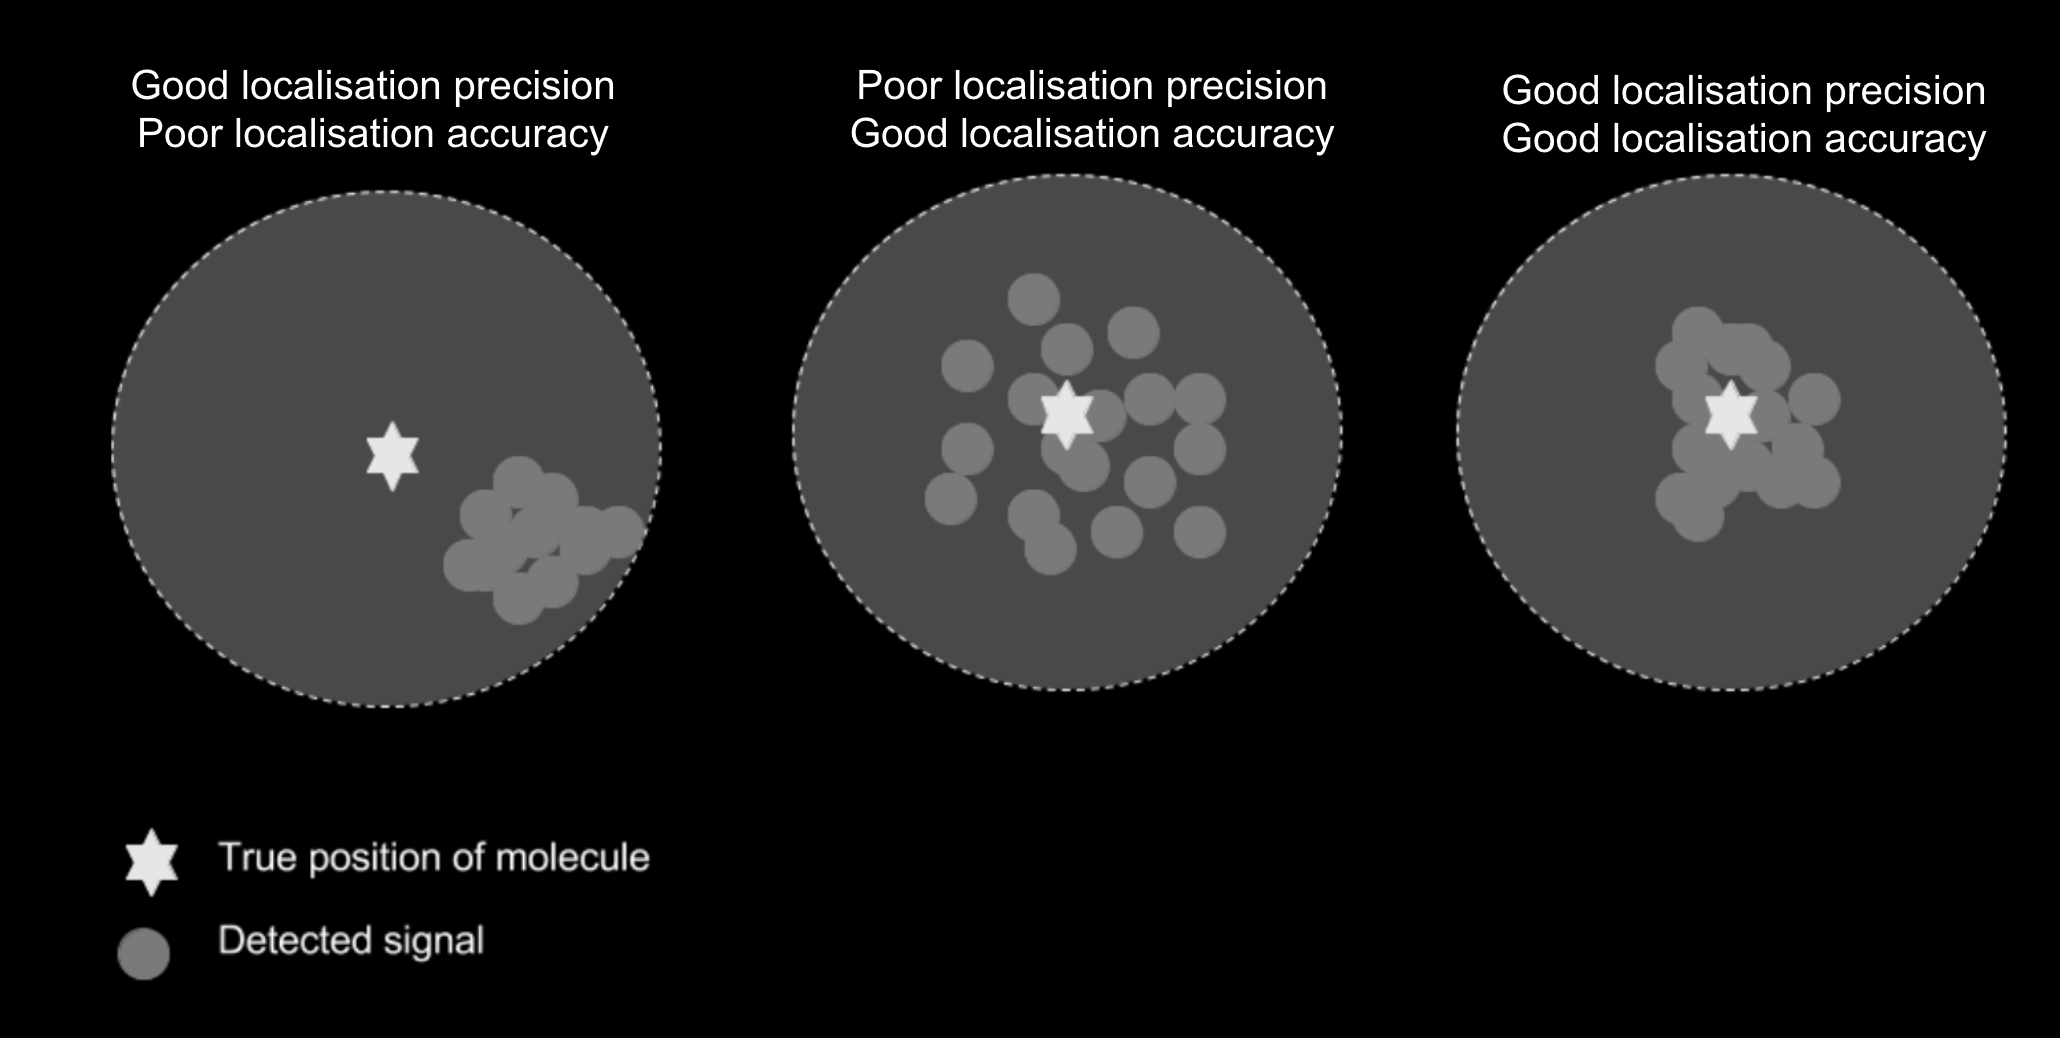
\includegraphics[width=15cm]{Figures/lp}
\end{center}
\caption[]{\textbf{Localisation precision of the fluorophore or the protein of interest:} The readers of super-resolution microscopy papers should look out when localisation precision is implied for spatial resolution. Resolution primarily depends on how densely a biological sample is labelled while localisation precision implies how well these labels are detected.
} \label{fig:lp}
\end{figure}


\end{document}



